\section{Introduction}
% With the broader coverage of online shopping across people in different ages and occupations, shopping demand varies for specific group of people or at specific period of time. In big companies, the traditional all-in-one shopping business pattern prone to be substituted by multiple business lines serving for people with distinct purposes. For example, 
% \KZ{This para is not well written.
% Go directly to explain what's product categorization and what it means by dynamic taxonomy scenario. No need to beat around the bush. One para on traditional problem and one para on the new problem will do. Now is too long! Don't introduce new names and acronyms at the beginning of the paper, especially the abstract. Use very easy to understand language.} When a broader coverage people embracing online shopping in recent years, numerous sellers swarm into e-commerce platforms with a surge of various kinds of products. 
% While the number of products keeps rising, it poses a bigger challenge for sellers to assign them with category tags and for platforms to manually organize them into category taxonomies as well. 
% Thus e-commerce platforms aim to train a model that automatically categorizes products and provide suggestions for those sellers, in order to improve their user experience.

% Typically product categories are organized into a hierarchical structure and 
Product categorization \cite{ding2002goldenbullet} is a specific text classification task that classifies product titles or descriptions into a pre-defined taxonomy of category nodes.
% , using their description texts such as titles. 
With the growth of businesses, 
% a real world and more challenging scenario is faced by 
giant e-commerce platforms (\textit{e.g.,} Amazon and Alibaba) are facing more complicated scenario. We define it as \textit{Dynamic Multi-Domain Product Categorization (DMPC)} 
, depicted in \figref{fig:teaser}, which simultaneously considers \textbf{multi-domain taxonomies} and \textbf{taxonomy evolving} challenges.

% For example, a product named \textit{``Red Wine Flavor Ice Cream $60g \times 6$''} should be categorized into 
% % \textit{"Dairy Food $\rightarrow$ Frozen $\rightarrow$ Ice Cream"}.
% \verb|Dairy Food| $\rightarrow$ \verb|Frozen| $\rightarrow$ \verb|Ice Cream|.
% It is also a crucial part of product understanding in which the accurate categorization of products further provides guidance for other e-commerce application scenarios, such as the user query navigation or advertisement recommendation. 

% Unlike vanilla text classification tasks, product categorization in e-commerce scenarios deals with thousands of fine-grained leaf node categories, which is known as the \textbf{large label space} challenge.
% % For example in Meituan e-commerce platform, there are an average -- newly uploaded products per day. 
% Although plenty of works concentrate on this challenge and formulate it as a multi-class hierarchical classification task with a fixed set of labels~\cite{kozareva2015everyone, cevahir2016large}, they ignore the situation where there exists multiple category taxonomies from different business lines and they will continuously evolve. 

\begin{figure}[tbp]
  \centering
  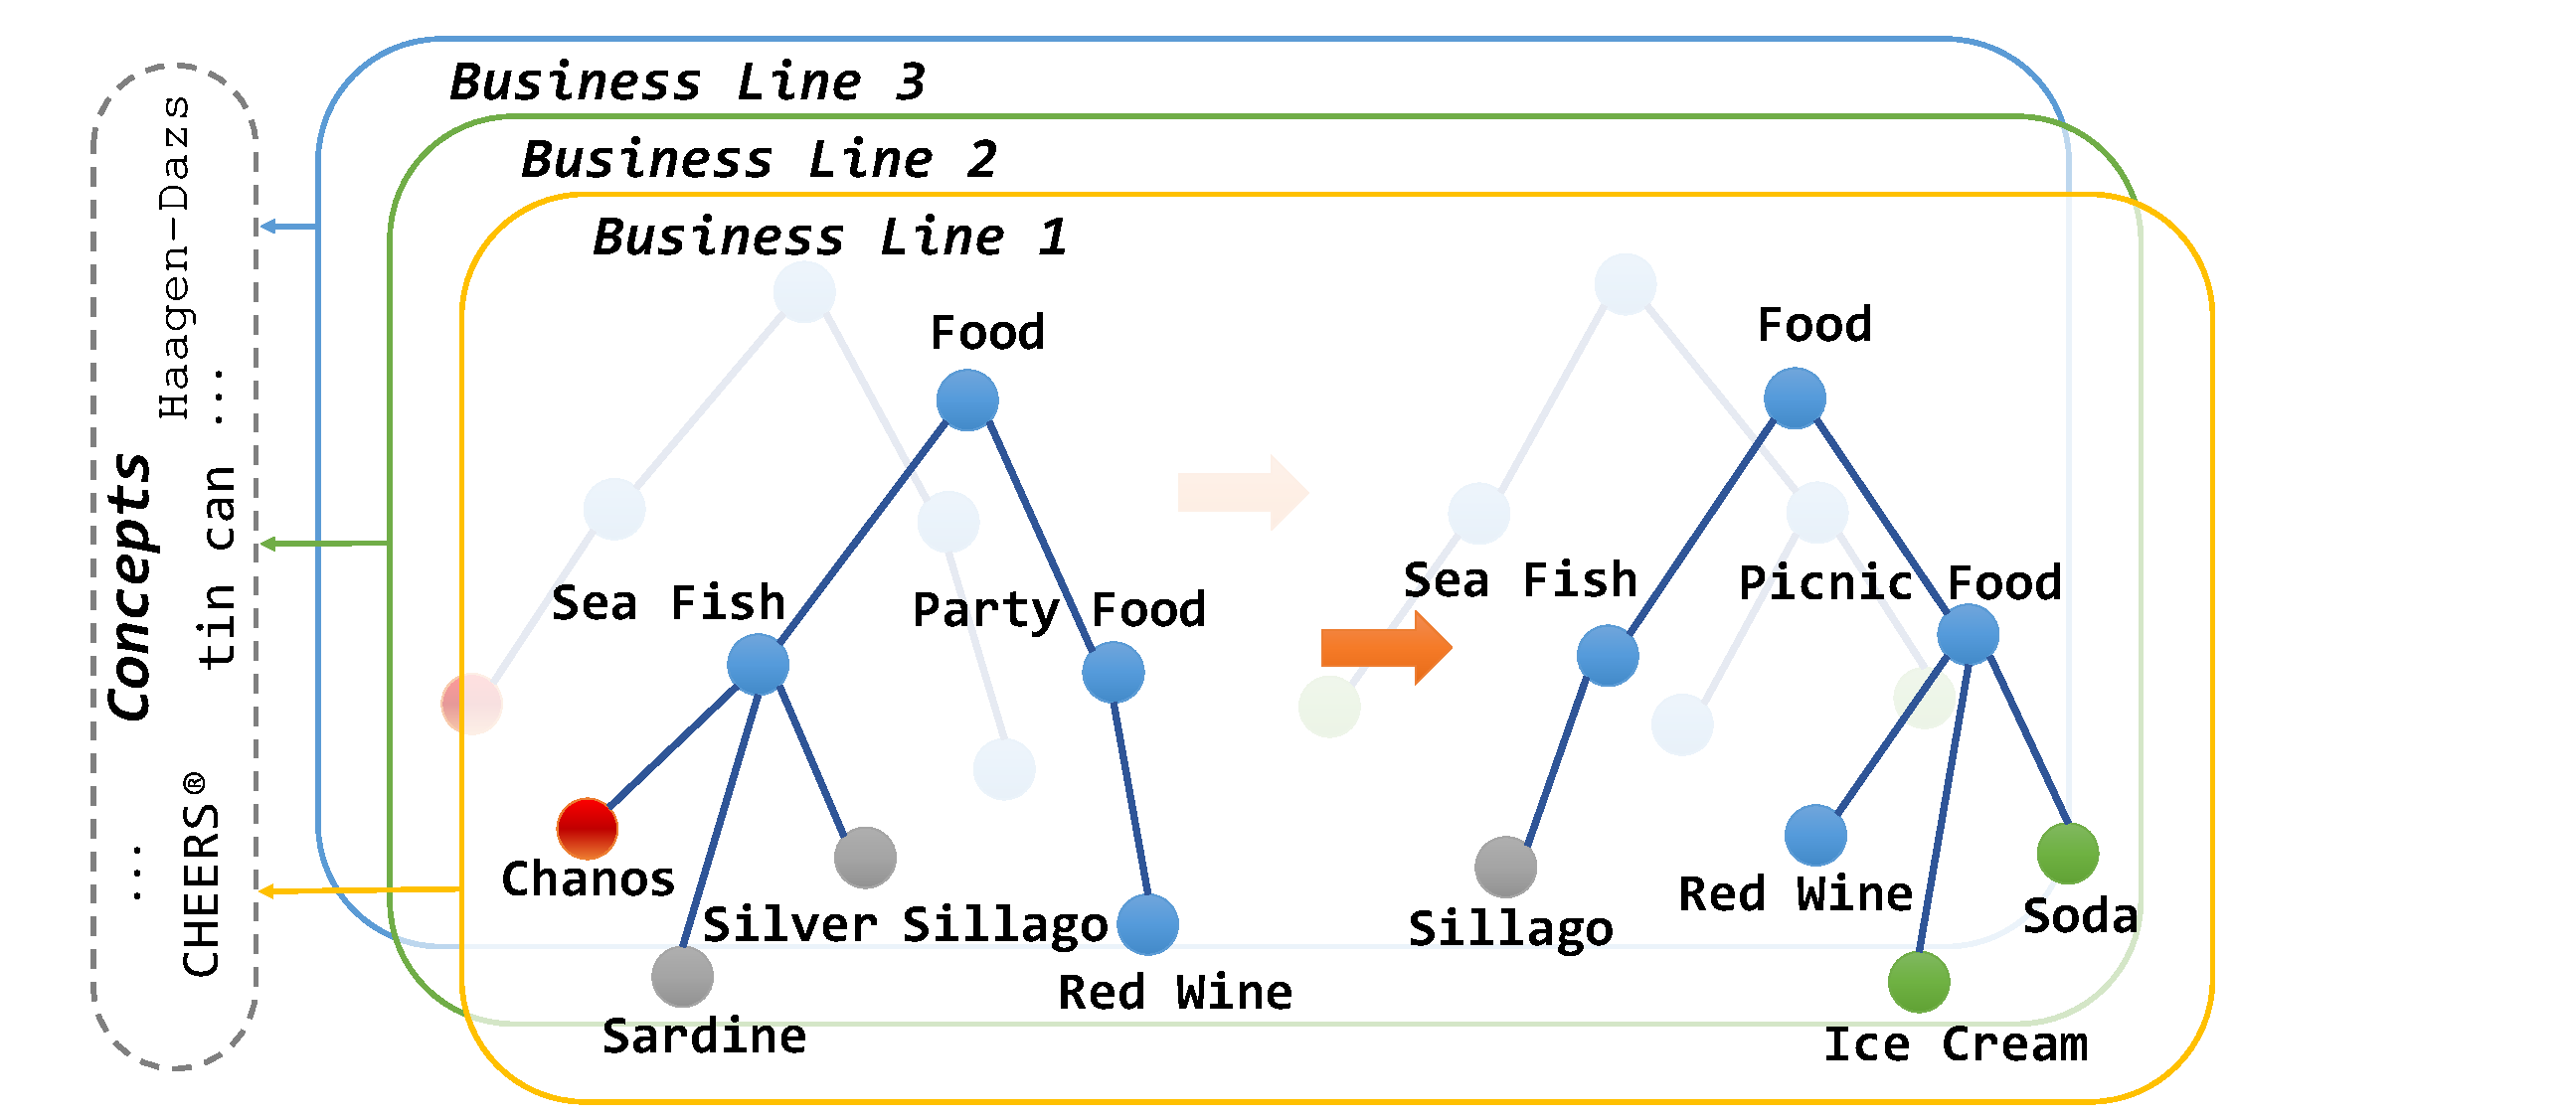
\includegraphics[width=\linewidth]{fig1}
  \caption{
%   An illustration of multiple taxonomies and taxonomy evolving. 
  Multiple taxonomies from different business lines are evolving themselves, including node deletion, integration, increment, and so on. But the fine-grained concepts of products seldom shift. }
  \label{fig:teaser}
\end{figure}

% A real world dilemma is that 
In real world scenarios, e-commerce platforms usually maintain \textbf{multiple} business lines with relatively independent \textbf{taxonomies}.
% and their corresponding \textbf{taxonomies}.
% but share a part of similar products. 
These business lines are catering for different customer demands or 
% fine-grained business domains, 
specific domain applications, 
for example, one provides fast delivery while another specializes in lower prices.
Multiple business domains correspond to different category label tree structures, with various depths and distinct literal expressions of tree nodes. 
% In addition, these models trained on specific category structures are incapable of extrapolating to another taxonomy categorization task. 

Meanwhile, with the expansion and reorganization of businesses, one category \textbf{taxonomy} keeps \textbf{evolving} as well, where 
% the expression of categories may change 
old categories might be deleted or integrated and new categories are possibly added.
% As is shown in \figref{fig:teaser}, when a minor business adjustment happens, \verb|Sardine| and \verb|Silver Sillago| are integrated into one category \verb|Sillago|, while \verb|Chanos| is removed and \verb|Fish Roe|, \verb|Sashimi| are added to the taxonomy. 
Conventional classifiers should be re-trained every time taxonomy changes, which is less robust towards taxonomy evolving issues.
% On the one hand, 
While training and maintaining separate models for each domain is laborious, 
% On the other hand, 
rich resources in cross-domain data 
and the inside knowledge 
are hardly exploited as well.
In \textit{DMPC} settings, a qualified system is supposed to tackle the dynamic label space and sustains accuracy in zero-shot conditions.
% We call this the challenge of \textbf{evolving taxonomy}.

\cut{%%%%%%%%%%% No need the following summary %%%%%
To sum up, the challenges behind product categorization of giant e-commerce platforms are listed below.  
% \KZ{These challenges should be illustrated using some lively examples.}

\begin{enumerate}
    \item \textbf{Large label space}, a fundamental challenge that has been well studied in former works. They either use a flat classifier treating all leaf nodes equivalently \cite{yu2012product, ha2016large, das2016large, krishnan2019large, lee2020cbb, yang2020bert}, or follow the hierarchy structure to classify from coarse to fine level nodes \cite{hasson2021category, li2018don}.
    \item \textbf{Multi-domain taxonomies}. This is mostly studied in the multi-task learning paradigm \cite{liu-etal-2019-multi}, which manipulates different tasks with a joint model. However, it lacks the ability to tackle taxonomy evolving issues.
    \item \textbf{Taxonomy evolving}. Authors in \cite{xu2019open} formulated an open-world learning problem in which a model should reject unseen classes and learn to recognize new classes incrementally. Nonetheless, conditions, when classes are integrated or divided apart, are ignored in their work.
\end{enumerate}
}%%%%%%%%%%%%%%%

% To our best knowledge, there is no solution in e-commerce that could apply for all the three challenges.
% Derived from the above scenarios in production, we define the problem in which the above three challenges are considered simultaneously as Dynamic Multi-Domain Product Categorization (DMPC) problem. 
% In this work, we propose a unified framework named \textit{Taxonomy-agnostic Label Retrieval (TaLR)} to solve the problem above.
Intuitively, we reformulate such a dynamic classification problem as a label ranking problem in order to jointly circumvent the above issues.
% in \textit{DMPC} problem. 
We propose a two-stage \textit{Taxonomy-agnostic Label Retrieval (TaLR)} framework capturing the semantic relatedness between a product title and its corresponding category texts in vector space. 
To ensure both accuracy and efficiency, candidate categories are first retrieved and then reranked for the final prediction.
% the semantic similarity between product titles and category label texts.
This reformulation is especially beneficial for evolved and zero-shot categories when textual semantics are incorporated. 
For example, despite the integration of [$\mathtt{Sardine}$] and [$\mathtt{Silver}\,\mathtt{Sillago}$] into [$\mathtt{Sillago}$], their textual meanings are barely drifted.
% , and the meaning of incoming class labels like [$\mathtt{Fish Roe}$] and [$\mathtt{Sashimi}$] could be captured in textual semantics as well. 

However, pure textual matching approaches are insufficient for accurate categorization when some hidden concept knowledge is ignored.
For example, \textit{Haagen-Dazs Red Wine Flavor} might be wrongly categorized into [$\mathtt{Red\,Wine}$] instead of the correct [$\mathtt{Ice\,Cream}$], mainly because the keyword \textit{Red Wine} in the lexical surface form 
\textbf{dominates other information} in the semantic matching score and thus 
leads the model to a skewed direction. Here, \textit{Haagen-Dazs} is one of the fine-grained concepts which are easily ignored by pure semantic matching.
% in general semantic space.

Therefore we consider integrating concept knowledge into semantic vector space in both stages of \textit{TaLR} framework. 
% Since our concepts are constructed over all domains, the knowledge from \textbf{multi-domain taxonomies} can be jointly leveraged when we jointly training. 
% The concept knowledge is utilized in both stages of \textit{TaLR}. 
Specifically, in the retrieval stage, we devise a heuristic strategy to establish the mapping between concept knowledge and candidate categories.
% we design a heuristic strategy to ensemble the vector matching candidates. 
In the reranking stage, concept knowledge is incorporated with category labels as supervision signals for the contrastive pretraining of the scoring model.
In conclusion, our contributions are:

\begin{itemize}
    \item We are the first to address \textit{DMPC} problem and propose a unified \textit{TaLR} framework in general semantic space, which is robust and efficient to handle multiple taxonomies and taxonomy evolving issues (zero-shot). Corresponding multi-domain datasets will be released.
    % while incurs low operation \& maintenance cost and gives rise to low response latency. (\secref{sec:all res}, \secref{sec:time cons})
    % \item We leverage the contrastive information from inter-class and intra-class product titles to effectively boost the product understanding  of the model. 
    \item Our \textit{TaLR} framework integrates the concept knowledge from multiple domains by heuristically retrieving candidates and contrastive grouping products to enhance the semantic space of texts.
    % by jointly leveraging the concept knowledge from multiple domains.
    % Specifically, we propose the concept-enhanced retrieval strategy and integrate contrastive information from the inter- and intra-concept of products.

    \item Experiments on our collected three real-world product categorization datasets show
    % the advantage of integrating concepts and 
    \textit{TaLR} is able to effectively transfer knowledge across different domains. The unified \textit{TaLR} model outperforms three separately-trained SOTA classifiers by 2.1\% on overall accuracy and beats the multi-task model by 18.2\%. 
\end{itemize}